
\part{Infrastructure as a Service -- IaaS}
\section{Infrastructure as a Service -- Amazon Web Service}

AWS is distributed among \textbf{regions}. Each region is \textbf{isolated} for \textbf{fault tolerance and stability}. Each region consists of \textbf{availability zones} (eg: data centers), where data can be \textbf{replicated}. 

\begin{itemize}
	\item region availability: 99.99\% from Amazon's SLA(service level agreement). To profit from SLA, data must be replicated over at least 2 zones in case of failure.
	\item IaaS service model:
	\begin{itemize}
		\item compute: EC2,
		\item network: VPC, CloudFront
		\item storage: S3, EFS, EBS, instance storage
	\end{itemize}
\end{itemize}

\subsection{Compute Service: Elastic Compute Cloud EC2}
\begin{itemize}
	\item \textbf{virtual machine instance} running based on an AMI
	\item \textbf{Amazon Machine Image}: a copy of server with OS and preinstalled software (eg: Ubuntu server 18.04 LTS, SSD volume type)
	\item instance attached \textbf{ephemeral storage, block storage and virtual firewall}
	\item resource allocation through Xen Hypervisor (\textbf{bare metal hypervisor}) 
	\item \textbf{elastic IP address} possible: private \& public IP address \textbf{remains same} after start/stop 
	\item lifecycle: pending -- running -- stopping -- stopped --shutting down -- terminated
\end{itemize}

Comparison Amazon EBS-Backed \& Instance Store-Backed EC2 instance:

\begin{table}[H]
	\begin{center}
	\begin{tabular}{|l|p{5cm}|p{5cm}|}
		\hline
		Characteristics  &EBS-Backed  & Instance Store-Backed \\ \hline
		root device volume        &EBS volume  & Instance store volume   \\ \hline
		stopped state     & stop-state exists, restart at a different server possible  & no stop-state, only termination    \\ \hline
		data persistence       & lost when termination, kept in EBS when stopped  & lost when termination   \\ \hline
		modification  & modifiable at stop-state  & fixed    \\ \hline
	\end{tabular}
\end{center}
\end{table}

\subsection{Storage}
\begin{itemize}
	\item \textbf{Elastic Block Storage (EBS)}
	\begin{itemize}
		\item similar to Storage Area Network (SAN)
		\item can be \textbf{mounted into VM}
		\item multiple block storage can be \textbf{combined into RAID}
		\item \textbf{snapshots} of the block storage are \textbf{stored in S3 for backup or replication}
	\end{itemize}
	\item \textbf{EC2 instance storage}: 
	\begin{itemize}
		\item disk or SSD connected to the physical machine
		\item \textbf{data erased} when instance is \textbf{stopped or terminated}
	\end{itemize}
	\item \textbf{Elastic File System (EFS)}: 
	\begin{itemize}
		\item similar to Network Attached Storage (NAS), scalable
		\item can be created and mounted into VM
		\item files can be \textbf{shared among instances}
	\end{itemize}
	\item \textbf{Simple Storage Service (S3)}
	\begin{itemize}
		\item large size storage (up to 5TB)
		\item \textbf{slower access} compared to EBS or local disks, \textbf{high durability, low availability}
		\item Use-case: backup
	\end{itemize}
\end{itemize}

\begin{figure}[H]
	\centering
	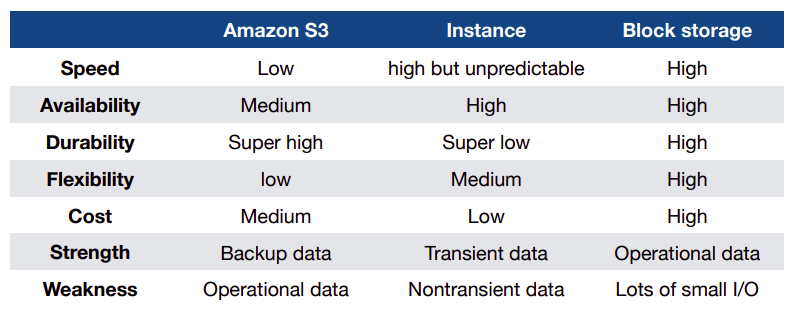
\includegraphics[width=0.8\textwidth]{awsstorage.png}
\end{figure}

Storage attached to EC2:
\begin{itemize}
	\item root device volume: EBS, instance storage. 
	\begin{itemize}
		\item instance stops: data \textbf{preserved}
		\item instance terminates: data \textbf{deleted}
	\end{itemize}
	\item instance store volume: local disks of the server. Data \textbf{erased} if instance stops
	\begin{itemize}
		\item instance stops: data \textbf{erased}
		\item instance terminates: data \textbf{erased}
	\end{itemize}
\end{itemize}

\subsection{Network}
\begin{itemize}
	\item \textbf{elastic IP address}: public IP address \textbf{remains same} even after start/stop.
	\item \textbf{Virtual Private Cloud (VPC)}: 
	\begin{itemize}
		\item resembles network in own data center, resources are launched into own VPC
		\item configuration of IP address range, subnets, route tables, network gateways, firewall settings	
	\end{itemize}
	\item \textbf{CloudFront}: content distributed network
	\begin{itemize}
		\item automatic distribution: content changes in S3 and will be automatically updated in every data center from edge locations
		\item response delivered from data center closed to requester.
	\end{itemize}
\end{itemize}


\section{Cloud Storage Systems}
\begin{itemize}
	\item Comparison VM storage VS. Cloud storage:
	\begin{itemize}
		\item VM: instance volume -- lost when VM stops, EBS volume -- lost when VM terminates.
		\item Cloud storage: for voluminous data potentially long-term storage.
	\end{itemize}
	\item requirements:
	\begin{itemize}
		\item voluminous data
		\item commodity hardware
		\item distributed data
		\item failures is norm rather exception: replication \& fault tolerance
		\item processed by application
		\item optimized for typical access patterns
	\end{itemize}
	\item \textbf{CAP Theorem}: aim for \textbf{availability} or \textbf{consistency}. Partition-tolerance has to be guaranteed.
	\item Types:
	\begin{itemize}
		\item object storage: S3
		\item shared file systems: NAS, EFS
		\item relational databases
		\item noSQL databases
		\item Data warehouse
	\end{itemize}
\end{itemize}

\subsection{Object Storage: AWS S3}
\begin{itemize}
	\item Goal: infinite data \textbf{durability} by 99.99\% availability
	\item Use-case: short-term or long-term \textbf{backup}
	\item storage classes:
	\begin{itemize}
		\item standard: for \textbf{frequently accessed} data
		\item reduce redundancy: for \textbf{reproducible, infrequently accessed} data
		\item intelligent tiering: objects are \textbf{automatically moved} between frequent and infrequent access tier.
		\item glacier: long-term data archive. long retrieval time
		\item deep-archive: even longer retrieval time, for \textbf{rarely accessed} data.
	\end{itemize}
	\item Data access: objects can be uploaded, retrieved and deleted. \textbf{No modification}.
	\item Versioning: versioning for individual files or entire buckets.
	\item Lifecycle: consists of rule that triggers \textbf{transition} to other storage classes or \textbf{expiration} of objects.
	\item consistency: \textbf{eventual consistency}. simultaneous puts -- last write wins.
\end{itemize}


\subsection{File Storage: Google File System}

\begin{itemize}
	\item \textbf{distributed} file system
	\item architecture:
	\begin{itemize}
		\item 1 \textbf{master server} + many \textbf{chunk servers}
		\item \textbf{master server}: metadata in main memory stored as \textbf{lookup table}
		\item \textbf{chunk server}: stores many 64MB-chunks as linux files.
		\item shadow masters possible to reduce load on master server
		\item \textbf{decoupled} control and data flow. \textbf{Control flow runs through master server} to chunk server, \textbf{data can directly flow from chunk server to client}.
	\end{itemize}
	\item replication: data is replicated to balance workload and combat failures.
	\item data access: client \textbf{first contacts master server} and finds out the corresponding chunk server through lookup table. Later interactions(writes, read) \textbf{directly between chunk and client}. 
	\item consistency: cocurrent writes possible, but only writes on \textbf{primary chunk} will be \textbf{replicated}. \textbf{consistent but undefined state}.
	\item Limitations:
	\begin{itemize}
		\item scalability of single master $\rightarrow$ development of distributed master
		\item fixed chunk size, while application can have smaller files.
		\item no latency guarantees.
	\end{itemize}
	\item other file systems: AWS Elastic File System
\end{itemize}

\subsection{Relational Database}

\begin{itemize}
	\item data represented as \textbf{n-ary relations}. Each relation is a \textbf{table}, which is defined by \textbf{schema}.
	\item data access: SQL-queries
	\item \textbf{ACID-properties} of transactions: atomicity, consistency, isolation, durability
	\item designed for \textbf{vertical scaling}
	\item Installation of own database:
	\begin{itemize}
		\item installation and management \textbf{on you own}
		\item data management: certificate, patching, performance tuning, backup, scaling, security 
	\end{itemize}
	\item Cloud relational database service: Amazon \textbf{managed} RDS, Amazon Aurora (own relational database)
	\begin{itemize}
		\item \textbf{managed} standard relational databases: mySQL, PostgreSQL
		\item different \textbf{certifications provided}
		\item \textbf{pre-configured} database instances
		\item standby copies in case of failovers
		\item multiple read replicas to increase read throughput, guarantee fault tolerance
		\item \textbf{automatic} backup snapshots in S3, \textbf{automatic} scaling
	\end{itemize}
\end{itemize}

\subsection{NoSQL Database}

\begin{itemize}
	\item database for \textbf{non-relational} data \textbf{without predefined schema}. Easy to define new attributes.
	\item designed for \textbf{horizontal scaling}
	\item Types of NoSQL databases:
	\begin{itemize}
		\item key-value database: Amazon Dynamo
		\item document oriented
		\item graph database
	\end{itemize}
	\item Cloud NoSQL database service: Amazon Dynamo DB
	\begin{itemize}
		\item \textbf{distributed} data store $\rightarrow$ optimized for \textbf{small} request, \textbf{quick} access and \textbf{high availability}.
		\item \textbf{key-value} database
		\begin{itemize}
			\item \textbf{primary key}: unique for each row, \textbf{composite key} possible (partition key + sort key).
			\item values: a set of attributes
		\end{itemize}
		\item Consistency: \textbf{eventual consistency}
		\begin{itemize}
			\item \textbf{normal reads}: eventual consistency, might return old values
			\item \textbf{strong consistent reads}: consistent, always the latest.
		\end{itemize}
		\item Architecture:
		\begin{itemize}
			\item \textbf{key-value pairs} stored in \textbf{tables}. 
			\item \textbf{tables} stored in \textbf{partitions}
			\item number of partitions depends on: size, required read/write capacity units
		\end{itemize}
		\item management of partitions: key $\rightarrow$ partition $\rightarrow$ virtual node $\rightarrow$ physical nodes
		\begin{itemize}
			\item key $\rightarrow$ partition: key-value pair entries are \textbf{hashed by keys} onto a \textbf{ring space} of partitions.
			\item partition $\rightarrow$ node: \textbf{ring} is split into \textbf{segments containing multiple partitions}. Each segment is managed by a \textbf{virtual node}.
			\item virtual node $\rightarrow$ physical node
		\end{itemize}
		\item Replication: (N, R, W)
		\begin{itemize}
			\item N: replication to \textbf{N consecutive nodes}. N $\uparrow$, durability $\uparrow$
			\item R: success \textbf{read} on \textbf{R copies}. R $\downarrow$, latency $\uparrow$
			\item W: success \textbf{write} on \textbf{W copies}. W $\downarrow$, latency $\uparrow$
			\item \textbf{R + W > N}: ensures the \textbf{most recent write} is returned.
		\end{itemize}
		
		\item Failures is a \textbf{norm}: \textbf{gossip protocol}
		

	\end{itemize} 
\end{itemize}

